% no notes
\documentclass{beamer}
% notes and slides
%\documentclass[notes]{beamer}
% notes only
%\documentclass[notes=only]{beamer}
\usepackage{graphicx} % Allows including images
\usepackage{booktabs} % Allows the use of \toprule, \midrule and \bottomrule in tables
\usepackage{multirow}
\usepackage{multimedia}
\usepackage{tikz}
\usepackage{circuitikz}
\usepackage{url}
\usepackage{pgfplots}
\pgfplotsset{compat=newest}
\usepgfplotslibrary{groupplots,dateplot}
\usetikzlibrary{patterns,shapes.arrows}
\usepackage{standalone}
\usepackage{adjustbox}
\usepackage{lmodern}
\usepackage{pgfplots}
\usepackage{amsmath}
\usepackage{amsthm}
\usepackage{multimedia}
\usepackage{standalone}
\usepackage{csquotes}
\usepackage{caption}
%\usepackage{hyperlink}
%\usepackage{url}

% python listings
% from https://tex.stackexchange.com/questions/83882/how-to-highlight-python-syntax-in-latex-listings-lstinputlistings-command
% Default fixed font does not support bold face
\DeclareFixedFont{\ttb}{T1}{txtt}{bx}{n}{12} % for bold
\DeclareFixedFont{\ttm}{T1}{txtt}{m}{n}{12}  % for normal

% Custom colors
\usepackage{color}
\definecolor{deepblue}{rgb}{0,0,0.5}
\definecolor{deepred}{rgb}{0.6,0,0}
\definecolor{deepgreen}{rgb}{0,0.5,0}

\usepackage{listings}

% Python style for highlighting
\newcommand\pythonstyle{\lstset{
language=Python,
basicstyle=\ttm,
morekeywords={self},              % Add keywords here
keywordstyle=\ttb\color{deepblue},
emph={MyClass,__init__},          % Custom highlighting
emphstyle=\ttb\color{deepred},    % Custom highlighting style
stringstyle=\color{deepgreen},
frame=tb,                         % Any extra options here
showstringspaces=false
}}


% Python environment
\lstnewenvironment{python}[1][]
{
\pythonstyle
\lstset{#1}
}
{}

% Python for external files
\newcommand\pythonexternal[2][]{{
\pythonstyle
\lstinputlisting[#1]{#2}}}

% Python for inline
\newcommand\pythoninline[1]{{\pythonstyle\lstinline!#1!}}

\PassOptionsToPackage{american}{babel} % change this to your language(s), main language last
% Spanish languages need extra options in order to work with this template
% \PassOptionsToPackage{spanish,es-lcroman}{babel}
\usepackage{babel}

\PassOptionsToPackage{%
  backend=biber,bibencoding=utf8, %instead of bibtex
  %backend=bibtex8,bibencoding=ascii,%
  language=auto,%
  style=numeric-comp,%
  %style=authoryear-comp, % Author 1999, 2010
  %bibstyle=authoryear,dashed=false, % dashed: substitute rep. author with ---
  style=alphabetic,
  sorting=nyt, % name, year, title
  maxbibnames=10, % default: 3, et al.
  %backref=true,%
  %natbib=true % natbib compatibility mode (\citep and \citet still work)
}{biblatex}
\usepackage{biblatex}
% Redefine the caption format to remove "Figure"
\captionsetup[figure]{labelformat=empty}


\addbibresource{bib.bib}

\usetheme{metropolis}           % Use metropolis theme
\setbeamertemplate{caption}[default]
\title{Introduction to Neural Networks}
\date{February 24, 2025}%{\today}
%\institute{High-Performance Computing and Analytics Lab}
%\author{Moritz Wolter}
\institute{Visual Computing Group, University of Bonn}
\author{Elena Trunz}


\titlegraphic{
\includegraphics[width=2.00cm]{UNI_Bonn_Logo_Standard_RZ.pdf}}

\begin{document}
    \maketitle

    \begin{frame}
    \frametitle{Overview} 
    \tableofcontents
    \end{frame}

    \section{Neural networks}
    \begin{frame}{The wonders of the human visual system}
      \begin{figure}
        \includestandalone[width=0.9\linewidth,height=1.5cm]{./figures/mnist_sequence}
        \caption{Most humans effortlessly recognize the digits \texttt{5 0 4 1 9 2 1 3}.}
      \end{figure}
    \end{frame}

    \begin{frame}{Biological motivation}
      \centering
      \begin{figure}
        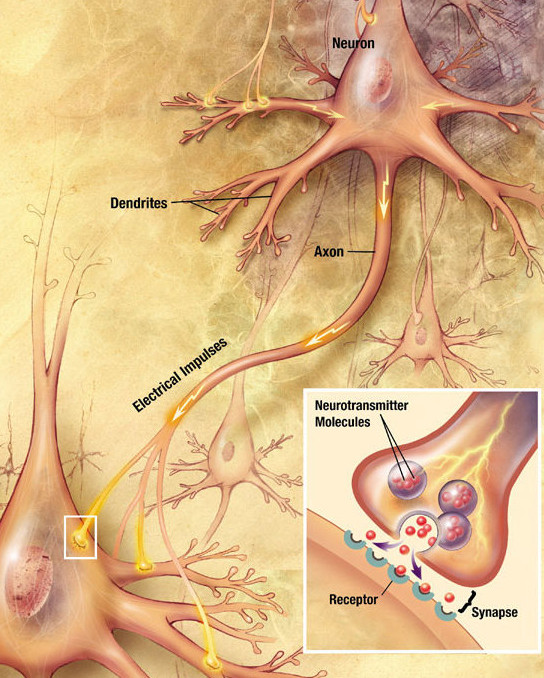
\includegraphics[scale=0.3]{./figures/Chemical_synapse_schema_cropped}  
      \end{figure}
      Image source: en.wikipedia.org
      %Image source: \url{https://en.wikipedia.org/wiki/Neuron#/media/File:Chemical_synapse_schema_cropped.jpg} 
    \note{
      \begin{itemize}
        \item A Human brain contains approximately 86 billion neurons.
        \item $10^{14}$ to $10^{15}$ synapses connect these neurons.
        \item Neurons receive inputs from dendrites.
        \item and can produce output signals along its axon.
        \item Axons connect neurons, modeled by weighting inputs $wx$.
        \item Neuron inputs can be inhibitive (negative weight) or
        \item excitatory (positive weight).
        \item If enough inputs excite a neuron, it fires.
        \item The activation function aims to mimic this behavior.
        \item Even though neural networks started out as biologically motivated,
        \item engineering efforts have since diverged from biology.
      \end{itemize}
    }
    \end{frame}


    \begin{frame}{The perceptron}
      Can computers recognize digits? Mimic biological neurons,
      \begin{figure}
        \includestandalone[scale=.575]{./figures/perceptron}
      \end{figure}
      Formally a single perceptron is defined as
      \begin{align}
        f(\mathbf{w}^T \mathbf{x} + b) = h
      \end{align}
      with $\mathbf{w} \in \mathbb{R}^n$, $\mathbf{x} \in \mathbb{R}^n$ and $h,b \in \mathbb{R}$. 
    \end{frame}

    \begin{frame}{The activation function $f$}
		 Activation functions should be differentiable and non-linear. Two popular choices for the activation function $f$ are
      \begin{figure}
				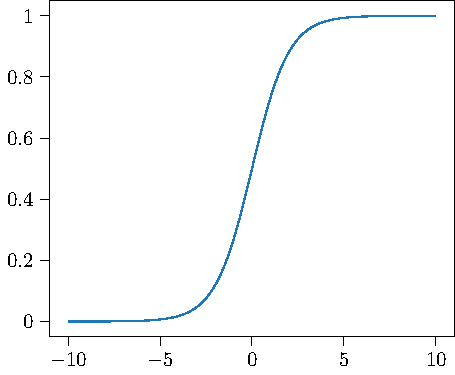
\includegraphics[width=0.49\linewidth]{./figures/sigmoid.pdf} 
				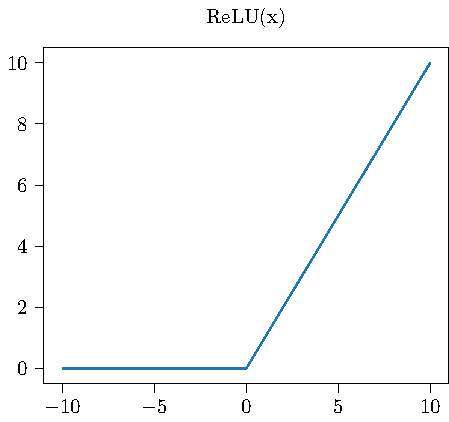
\includegraphics[width=0.49\linewidth]{./figures/relu.pdf} 
        %\includestandalone[width=0.49\linewidth]{./figures/sigmoid}
        %\includestandalone[width=0.49\linewidth]{./figures/ReLU}
      \end{figure}
    \end{frame}

    \begin{frame}{Fully connected layer}
      Let's extend the definition to cover an array of perceptrons:
      \begin{figure}
        \includestandalone[scale=0.5]{./figures/perceptron_array}
      \end{figure}
      Every input is connected to every neuron. In matrix language, this turns into
      \begin{align}
        \bar{\mathbf{h}} &= \mathbf{W}\mathbf{x} + \mathbf{b}, & \mathbf{h} = f(\bar{\mathbf{h}}).
      \end{align}
      With $\mathbf{W} \in \mathbb{R}^{m,n}$, $\mathbf{x} \in \mathbb{R}^{n}$, $\mathbf{b} \in \mathbb{R}^{m}$, and $\mathbf{h}, \bar{\mathbf{h}} \in \mathbb{R}^m$.
    \end{frame}
		
		\begin{frame}{Multi-layer networks}
      Stack dense (fully connected) layers and activations to create deeper networks. \\
      \begin{figure}
        \includestandalone[width=\linewidth]{./figures/multilayer1} 
      \end{figure}	%\pause
			The activation function used right before the output is typically chosen based on the nature of the task and often differs from those used in the hidden layers.
    \end{frame}
		
		\begin{frame}{Output activations}
      \begin{itemize}
				\item Regression: The activation function is simply an identity function, i.e. $h = \bar{h}$.	%\pause
				\item Classification: 
				\begin{itemize}
					\item Logistic sigmoid function for binary classification: 
						\[\sigma_{\text{binary}}(\bar{h}) = \frac{1}{1+\exp(-\bar{h})}\]
					\item  Soft-max activation for multiple classes: 
					\[ \sigma_{\text{multi-class}}(\bar{h}) = \frac{\exp(\bar{h}_c)}{\sum_b\exp(\bar{h}_b)}\]
				\end{itemize}
			\end{itemize}
    \end{frame}
		
		\section{Training neural networks}

    \begin{frame}{The loss function}
		\begin{itemize}
      \item To choose weights for the network, we require a quality measure.
      \item We already saw the mean squared error cost function:
      \begin{align}
        C_{\text{mse}} = \frac{1}{2} \sum_{k=1}^{n} (\mathbf{h}_k - \mathbf{y}_k)^2 = \frac{1}{2} (\mathbf{h} - \mathbf{y})^T(\mathbf{h} - \mathbf{y})
      \end{align}
      \item This function measures the squared distance from each desired output.
      $\mathbf{y}$ denotes the desired labels, and $\mathbf{h}$ represents network output.  %\pause
			\item We want to find the parameters $\mathbf{W}$ and $\mathbf{b}$ that minimize our loss. 
			\end{itemize}
    \end{frame}
		
		\begin{frame}{Optimization}
      \begin{itemize}
      \item We use gradient descent to minimize our loss function.
			\item That means we need to compute the gradients of the loss function with respect to each weight in the network. 
			\item These gradients will tell us how much each weight should change to reduce the overall error. %\pause
			\item How can we compute the gradients efficiently? %\pause
			\begin{itemize}
				\item[$\rightarrow$] We use \emph{backpropagation}
			\end{itemize}
			\end{itemize}
    \end{frame}
		
		\begin{frame}{Gradient descent with backpropagation}
    \begin{enumerate}
        \item Perform a forward pass through the network.
        \item Compute the gradient of the loss with respect to the output layer.
        \item Backpropagate the error through the network.
        \item Update the weights using the gradients.
				\item Repeat steps 1) - 4) until convergence.
    \end{enumerate}
		\note<1>{ 1) Compute the output of the network by passing the input through each layer to the final output layer.
		2) Using the derivative of the loss function, we measure how much the output layer contributed to the error (Calculate how much the loss changes with respect to the output of the network, which tells us how far the prediction is from the true value.) 
		3) Propagate the gradients backward through each layer, using the chain rule, to determine how each weight contributed to the error.
		4) Adjust the weights by a small amount in the opposite direction of the gradients to minimize the loss and improve the model (gradient descent)
		}
\end{frame}

\begin{frame}{Step 1: Forward pass}
   \begin{figure}
        \includestandalone[width=\linewidth]{./figures/multilayer1} 
      \end{figure}
	\end{frame}

\begin{frame}{Step 2: Gradient for output}
The gradient of the mse-cost-function: Both the mean squared error loss function and our dense layer are differentiable. 
\begin{align}
        \frac{\partial C_{\text{mse}}}{\partial \mathbf{h}} = \mathbf{h} - \mathbf{y} = \triangle_{\text{mse}}
      \end{align}
      The $\triangle$ symbol~\cite{nielsen2015neural} will re-appear. It always indicates incoming gradient information from above.
      If the labels are a vector of shape $\mathbb{R}^m$, $\triangle$ and the network output $\mathbf{h}$ must share 
      this dimension.
\note<1>{ Gradient of the loss function with respect to the output layer
		}
	\end{frame}
	
    %\begin{frame}{The gradient of the mse-cost-function}
      %Both the mean squared error loss function and our dense layer are differentiable. 
      %\begin{align}
        %\frac{\partial C_{\text{mse}}}{\partial \mathbf{h}} = \mathbf{h} - \mathbf{y} = \triangle_{\text{mse}}
      %\end{align}
      %The $\triangle$ symbol will re-appear. It always indicates incoming gradient information from above.
      %If the labels are a vector of shape $\mathbb{R}^m$, $\triangle$ and the network output $\mathbf{h}$ must share 
      %this dimension.
    %\end{frame}
		
		\begin{frame}{Step 3: Backpropagate the gradient}
		Recall the chain rule $(g(h(x)))' = g'(h(x)) \cdot h'(x)$. %\pause

		We use chain rule to backpropagate the gradient trough the activation function and the dense layer and repeat this for all layers down to the input.
	\end{frame}
	
	\begin{frame}{Step 3: Backpropagate the gradient: Activation}
		From the forward pass we have: $\mathbf{h} = f(\bar{\mathbf{h}})$. \\
		From backpropagation, we get an incoming gradient (error term) from the next layer:  
		\begin{align*}
        \frac{\partial C}{\partial \mathbf{h}} = \triangle
      \end{align*}
			We backpropagate it through the activation function:
			\begin{align*}
        \frac{\partial C}{\partial \bar{\mathbf{h}}} = \frac{\partial C}{\partial \mathbf{h}} \cdot \frac{\partial \mathbf{h}}{\partial \bar{\mathbf{h}}} = \triangle \odot f'(\bar{\mathbf{h}}),
      \end{align*}
			where $\odot$ is the element-wise product.
			\note{f'(\bar{\mathbf{h}} is the derivative of the activation function, which is why we need our activation function to be differentiable.}
	\end{frame}
	
	\begin{frame}{Step 3: Backpropagate the gradient: Dense layer}
		\begin{align*}
        \frac{\partial C}{\partial \mathbf{W}} = \frac{\partial C}{\partial \bar{\mathbf{h}}} \cdot \frac{\partial \bar{\mathbf{h}}}{\partial \mathbf{W}}, \quad \quad \frac{\partial C}{\partial \mathbf{b}} = \frac{\partial C}{\partial \bar{\mathbf{h}}} \cdot \frac{\partial \bar{\mathbf{h}}}{\partial \mathbf{b}}, \quad \quad \frac{\partial C}{\partial \mathbf{x}} = \frac{\partial C}{\partial \bar{\mathbf{h}}} \cdot \frac{\partial \bar{\mathbf{h}}}{\partial \mathbf{x}}
      \end{align*}
		From the forward pass we know: $\bar{\mathbf{h}} = \mathbf{W}\mathbf{x}+\mathbf{b}$. Thus:
		\begin{align*}
        \frac{\partial \bar{\mathbf{h}}}{\partial \mathbf{W}} =\mathbf{x}^T, \quad \quad \frac{\partial \bar{\mathbf{h}}}{\partial \mathbf{b}} =1, \quad \quad \frac{\partial \bar{\mathbf{h}}}{\partial \mathbf{x}} =\mathbf{W}
      \end{align*}
		Substituting:
		\begin{align*}
        \frac{\partial C}{\partial \mathbf{W}} = (\triangle \odot f'(\bar{\mathbf{h}}))\mathbf{x}^T, \quad \frac{\partial C}{\partial \mathbf{b}} = \triangle \odot f'(\bar{\mathbf{h}}), \quad \frac{\partial C}{\partial \mathbf{x}} = \mathbf{W}^T(\triangle \odot f'(\bar{\mathbf{h}}))
      \end{align*}
	\end{frame}

    %\begin{frame}{The gradient of a dense layer}
      %The chain rule tells us the gradients for the dense layer~\cite{nielsen2015neural}
      %\begin{align}
        %\delta \mathbf{W} &= [f'(\bar{\mathbf{h}}) \odot \triangle]\mathbf{x}^T, &  \delta \mathbf{b} = f'(\bar{\mathbf{h}}) \odot \triangle, \\
        %\delta \mathbf{x} &= \mathbf{W}^T [f'(\bar{\mathbf{h}}) \odot \triangle],
      %\end{align}
      %where $\odot$ is the element-wise product. $\delta$ denotes the cost function gradient for the value following it \cite{greff2016lstm}. \\
      %With $\delta \mathbf{W} \in \mathbb{R}^{m,n}$, $\delta \mathbf{x} \in \mathbb{R}^{n}$ and $\delta \mathbf{b} \in \mathbb{R}^{m}$.
      %\textbf{Modern libraries will take care of these computations for you!} \\
      %
      %\note<1>{
        %On the board, derive:
        %Recall the chain rule $(g(h(x)))' = g'(h(x)) \cdot h'(x)$.
        %For the activation function, we have,
        %\begin{align}
          %\mathbf{h} &= f(\bar{\mathbf{h}}) \\
          %\Rightarrow \delta \bar{\mathbf{h}} &= f'(\bar{\mathbf{h}}) \odot \triangle
        %\end{align}
        %For the weight matrix,
        %\begin{align}
          %\bar{\mathbf{h}} &= \mathbf{W}\mathbf{x} + \mathbf{b} \\
          %\Rightarrow \delta \mathbf{W} &= \delta \bar{\mathbf{h}} \mathbf{x}^T = [f'(\bar{\mathbf{h}}) \odot \triangle] \mathbf{x}^T
        %\end{align}
        %For the bias,
        %\begin{align}
          %\bar{\mathbf{h}}  &= \mathbf{W}\mathbf{x} + \mathbf{b} \\
          %\Rightarrow \delta \mathbf{b} &= 1 \odot \delta \bar{\mathbf{h}} = [f'(\bar{\mathbf{h}}) \odot \triangle]
        %\end{align}
      %}
    %\end{frame}
		
		\begin{frame}{The gradient of a dense layer}
      Let $\delta$ denote the cost function gradient for the value following it \cite{greff2016lstm}. It holds:
      \begin{align}
        \delta \mathbf{W} &= [f'(\bar{\mathbf{h}}) \odot \triangle]\mathbf{x}^T, &  \delta \mathbf{b} = f'(\bar{\mathbf{h}}) \odot \triangle, \\
        \delta \mathbf{x} &= \mathbf{W}^T [f'(\bar{\mathbf{h}}) \odot \triangle],
      \end{align}
      with $\delta \mathbf{W} \in \mathbb{R}^{m,n}$, $\delta \mathbf{x} \in \mathbb{R}^{n}$ and $\delta \mathbf{b} \in \mathbb{R}^{m}$.
      \textbf{Modern libraries will take care of these computations for you!} \\
    \end{frame}
		%
		\begin{frame}{Backpropagation}
      \begin{figure}
        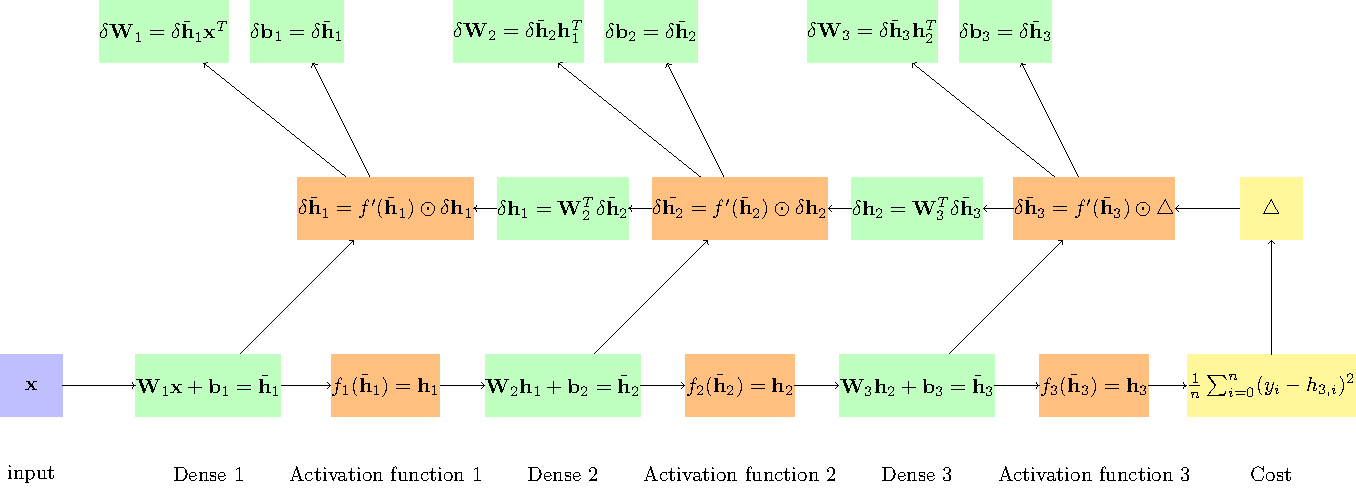
\includegraphics[width=\linewidth]{./figures/backprop.pdf} 
      \end{figure}
    \end{frame}
		
		\begin{frame}{Step 4: Updating the weights}
		The weights at the next time step $\tau + 1$ are given by,
		\begin{align*}
			\mathbf{W}_{\tau + 1} &= \mathbf{W}_\tau - \epsilon \cdot \delta\mathbf{W}_{\tau}, \\
			\mathbf{b}_{\tau + 1} &= \mathbf{b}_{\tau} - \epsilon \cdot \delta\mathbf{b}_{\tau},
			 \end{align*}
			where the step size, also called the learning rate, is given by $\epsilon \in \mathbb{R}$. At $\tau = 0$, matrix entries are random.
    \end{frame}
%
    \begin{frame}{Derivatives of our activation functions}
      \begin{align}
        \sigma'(x) = \sigma(x) \cdot (1 - \sigma(x)) \\
        \text{ReLU}'(x) = H(x) 
      \end{align}
      \begin{figure}
				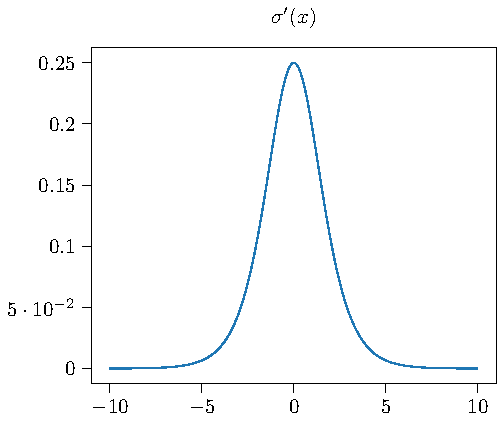
\includegraphics[width=0.49\linewidth]{./figures/sigmoid_prime.pdf} 
				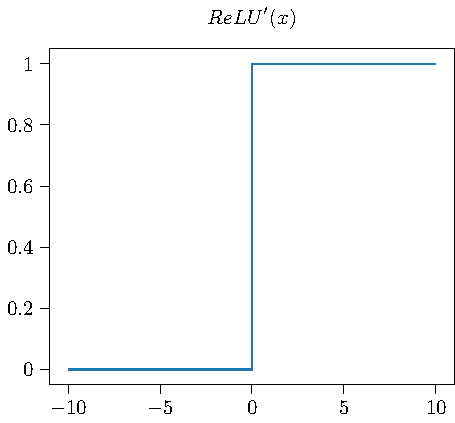
\includegraphics[width=0.447\linewidth]{./figures/relu_prime.pdf} 
        %\includestandalone[width=0.49\linewidth]{./figures/sigmoid_prime}
        %\includestandalone[width=0.447\linewidth]{./figures/relu_prime}
      \end{figure}
    \end{frame}

    \begin{frame}{Perceptrons for functions}
      The network components described this far already allow function learning.
      Given a noisy input signal $\mathbf{x} \in \mathbb{R}^{n}$ and a ground through output $\mathbf{y} \in \mathbb{R}^n$,
      define,
      \begin{align}
        \mathbf{h}_1 = \sigma(\mathbf{W}\mathbf{x} + \mathbf{b}) \\
        \mathbf{o} = \mathbf{W}_{\text{proj}}\mathbf{h}_1
      \end{align}
      With $\mathbf{W} \in \mathbb{R}^{m,n}$ and $\mathbf{b} \in \mathbb{R}^{m}$.
      $m$ and $n$ denote the number of neurons and the input signal length.
      For signal denoising, input and output have the same length.
      Therefore $\mathbf{W}_{\text{proj}} \in \mathbb{R}^{n,m}$.
      $\mathbf{o} \in \mathbb{R}^{n}$ denotes the network output.
    \end{frame}

    %\begin{frame}{Denoising a cosine}
      %Training works by iteratively descending along the gradients. For $\mathbf{W}$ the weights at the
      %next time step $\tau$ are given by,
      %\begin{align}
        %\mathbf{W}_{\tau + 1} = \mathbf{W}_\tau - \epsilon \cdot \delta\mathbf{W}_{\tau}.
      %\end{align}
      %The step size is given by $\epsilon \in \mathbb{R}$. At $\tau = 0$, matrix entries are random.
      %$\mathcal{U}[-0.1, 0.1]$ is a reasonable choice here.
      %The process is the same for all other network components.
    %\end{frame}

    \begin{frame}{Denoising a cosine}
			Here, the random initialization of the weights from $\mathcal{U}[-0.1, 0.1]$ is a reasonable choice.\\
      Optimization for 500 steps with 10 neurons, leads to the output below:
      \begin{figure}
        \includestandalone[width=.5\linewidth]{./figures/denoising}
        \caption{The cosine function is shown in blue, a noisy network input in orange, and a denoised network output in green.}
        \end{figure}
    \end{frame}

    \begin{frame}{Summary}
      \begin{itemize}
        \item Artificial neural networks are biologically motivated.
        \item Gradients make it possible to optimize arrays of neurons.
        \item A single array of layers of neurons can solve tasks like denoising a cosine.
      \end{itemize}
    \end{frame}


    \section{Classification with neural networks}

    %\begin{frame}{Deep multi-layer networks}
      %Stack dense layers and activations to create deep networks. \\
      %\begin{figure}
        %\includestandalone[width=\linewidth]{./figures/multilayer} 
      %\end{figure}
    %\end{frame}
%
    %\begin{frame}{Backpropagation}
      %\begin{figure}
        %\includestandalone[width=\linewidth]{./figures/backprop} 
      %\end{figure}
    %\end{frame}

    \begin{frame}{The cross-entropy loss}
      The cross-entropy loss function is defined as \cite{nielsen2015neural, bishop2006pattern}
      \begin{align} \label{eq:ce}
       C_{\text{ce}}(\mathbf{y}, \mathbf{o}) = -\sum_k^{n_o} [( \mathbf{y}_k  \ln \mathbf{o}_k) 
                                  + (\mathbf{1} - \mathbf{y}_k)
                                     \ln(\mathbf{1} - \mathbf{o}_k)].
      \end{align}
      With $n_o$ the number of output neurons. $\mathbf{y} \in \mathbb{R}^{n_o}$ the desired output and
      $\mathbf{o} \in \mathbb{R}^{n_o}$ the network output.
			\note{Cross-entropy is a good loss function for classification because it measures how different the predicted probability distribution is from the true distribution (i.e., the actual class labels). It works well because:

    Probabilistic Interpretation: Cross-entropy loss directly measures the dissimilarity between the predicted probability distribution and the true labels (which are one-hot encoded in classification tasks). This aligns with the goal of classification—to assign high probability to the correct class.

    Logarithmic Penalization: Cross-entropy applies a logarithm to the predicted probabilities, which strongly penalizes incorrect predictions with high confidence. This encourages the model to be confident only when it is correct.

    Better Gradient Properties: Compared to mean squared error (MSE), cross-entropy provides stronger gradients when the predictions are incorrect, leading to faster convergence during training.

    Naturally Works with Softmax: In multi-class classification, cross-entropy is often used with the softmax activation function, which turns logits into probabilities. The combination ensures that the loss function is well-behaved and suitable for optimizing probability distributions.

    Avoids Vanishing Gradients: Since cross-entropy loss does not have flat regions like MSE when used with sigmoid/softmax, it helps prevent vanishing gradients, ensuring efficient learning.}
    \end{frame}

    \begin{frame}{Understanding how cross-entropy works}
      To understand cross entropy let's consider the boundary cases $y=0$ and $y=1$.
      \begin{figure}
        \includestandalone[width=0.49\linewidth]{./figures/ce_label_0}
        \includestandalone[width=0.49\linewidth]{./figures/ce_label_1}
      \end{figure}
    \end{frame}

    \begin{frame}{Gradients and cross-entropy}
      If a sigmoidal activation function produced $\mathbf{o}$, the gradients can be computed using ~\cite{nielsen2015neural,bishop2006pattern}
      \begin{align} 
         \frac{\partial C_{ce}}{\partial \mathbf{h}} 
         = \sigma(\mathbf{o}) - \mathbf{y} = \triangle_{\text{ce}}
      \end{align}
      \note{
        Following \cite{nielsen2015neural}, substitute $\sigma(\mathbf{o})$ into eq~\ref{eq:ce}.
      }
    \end{frame}

    \begin{frame}{The MNIST-Dataset}
      \begin{figure}
        \includestandalone[width=0.9\linewidth,height=1.5cm]{./figures/mnist_sequence}
        \caption{The MNIST-dataset contains 70k images of handwritten digits.}
      \end{figure}
    \end{frame}

    \begin{frame}{Validation and Test data splits}
      \begin{itemize}
        \item To ensure the correct operation of the systems we devise, it is paramount to 
        hold back part of the data for validation and testing.
        \item Before starting to train, split off validation and test data.
        \item The 70k MNIST samples could, for example, be partitioned into 59k training images.
        1k validation images and 10k test images. 
      \end{itemize}
    \end{frame}

    \begin{frame}{Input-preprocessing}
      Standard initializations and learning algorithms assume an approximately standard normal distribution
      of the network inputs. Consequently, we must rescale the data using,
      \begin{align}
        {x}_{ij} = \frac{x_{ij} - \mu}{\sigma}
      \end{align}
      With $\mu$ and $\sigma$ the training set mean and standard deviation.
      For all pixels, $i,j$ up the height and width of every image.
      %$b$ denotes the number of data points, and $n$ is the data dimension.
    \end{frame}

    \begin{frame}{The effect of normalization}
      \begin{figure}
      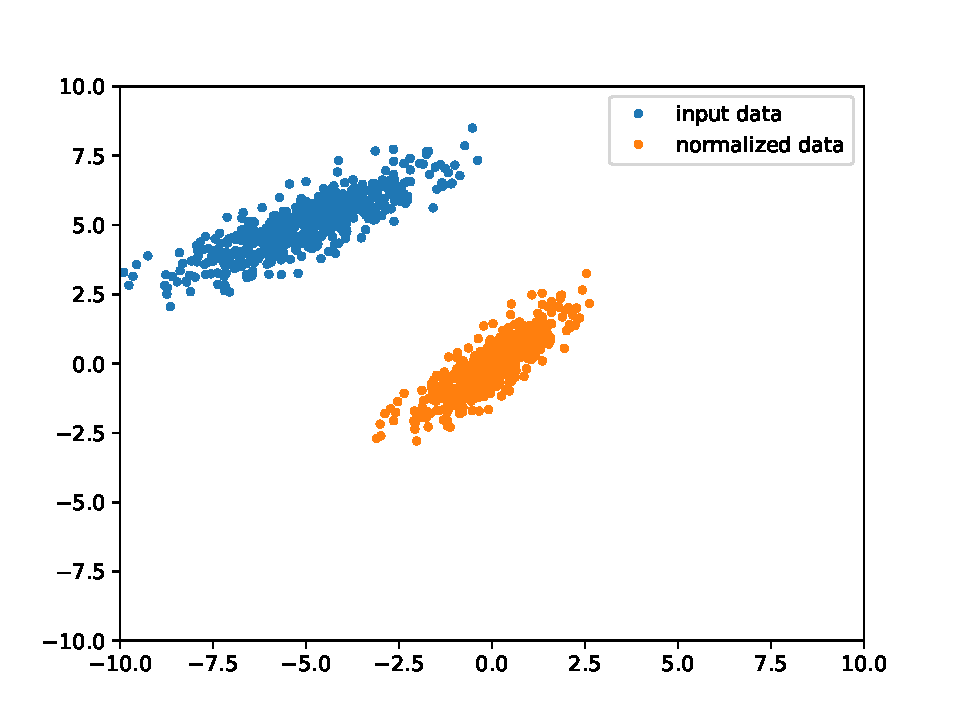
\includegraphics[width=\linewidth]{./figures/normalized.pdf}
      \end{figure}
    \end{frame}

    \begin{frame}{Whitening the inputs \cite{CS231n}}
      Instead of dividing by the standard deviation, rescale the centered data with the singular values of the covariance matrix.
      \begin{align}
        \mathbf{C} = \frac{1}{n} (\mathbf{x} - \mu)^T(\mathbf{x} - \mu)
      \end{align}
      With $n$ as the total number of data points. Next we find $\mathbf{U}\mathbf{\Sigma}\mathbf{V} = \mathbf{C}$.
      After projecting the data via $\mathbf{p} = \mathbf{x}\mathbf{U}$. Whitening now uses the singular values of $\mathbf{C}$ to rescale the data,
      \begin{align}
        p_{ij} = \frac{p_{ij}}{\sqrt{\sigma_j} + \epsilon}
      \end{align}
      With $\epsilon$ i.e. equal to $1e^{-8}$ for numerical stability.
      The operation is repeated for all pixel locations $i,j$ in the input image.
    \end{frame}

    \begin{frame}{The effect of Whitening}
    \begin{figure}
    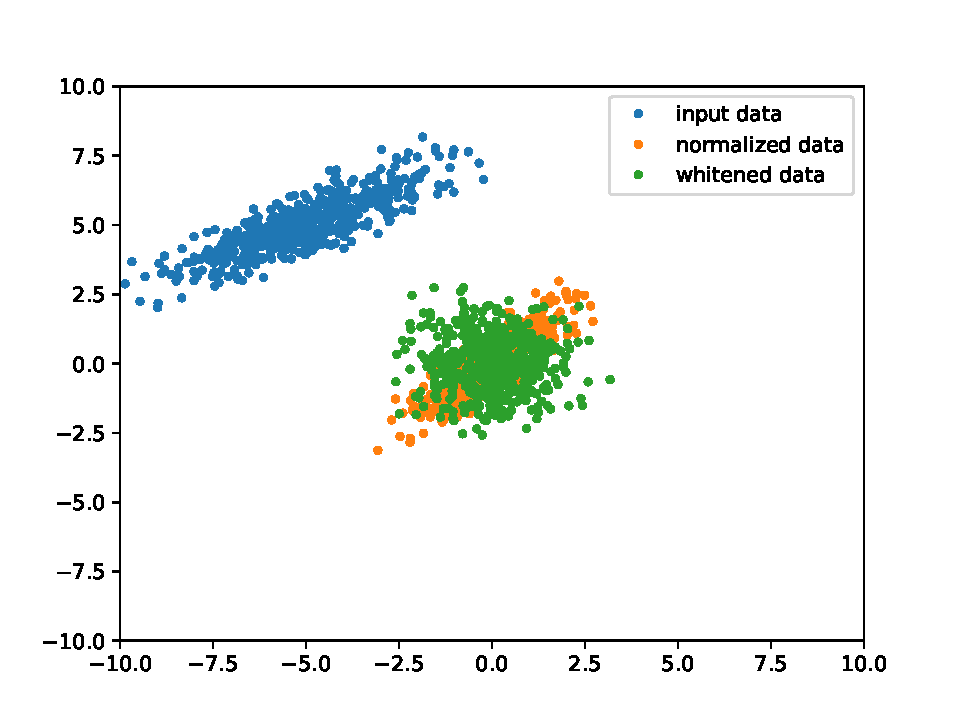
\includegraphics[width=\linewidth]{./figures/whitened.pdf}
      \end{figure}
      Whitening is expensive and sometimes unstable. Consequently, most projects rely on normalization.
    \end{frame}


    \begin{frame}{Label-encoding}
      It has proven useful to have individual output neurons produce probabilities for each class.
      Given integer labels $1,2,3,4, \dots \in \mathbb{Z}$. One-hot encoded label vectors have a one 
      at the label's position and zeros elsewhere. I.e.
      \begin{align}
        \begin{pmatrix}
          1 \\ 0 \\ 0 \\ 0 \\ \vdots
        \end{pmatrix},
        \begin{pmatrix}
          0 \\ 1 \\ 0 \\ 0 \\\vdots
        \end{pmatrix},
        \begin{pmatrix}
          0 \\ 0 \\ 1 \\ 0 \\\vdots
        \end{pmatrix},
        \begin{pmatrix}
          0 \\ 0 \\ 0 \\ 1 \\\vdots
        \end{pmatrix},
        \dots
      \end{align}
      for the integer label sequence above.
    \end{frame}


    \begin{frame}{Batching the data}
      Working with individual data points is not efficient in practice.
      Instead, we would like to process multiple (i.e. 64) samples in parallel. 
      Add a leading batch dimension and rely on broadcasting.

      An additional mean converts the cost of a batch into a scalar.
      In the cross-entropy case:
      \begin{align}
        C_{\text{ce}}(\mathbf{y},\mathbf{o})=-\frac{1}{n_b}\sum_{i=1}^{n_b}\sum_{k=1}^{n_o}[(\mathbf{y}_{i,k}\ln\mathbf{o}_{i,k})+(\mathbf{1}-\mathbf{y}_{i,k})\ln(\mathbf{1}-\mathbf{o}_{i,k})]
      \end{align}
      With $n_o$ the number of output neurons and $n_b$ the batch size.
    \end{frame}

    \begin{frame}{MNIST-Classification}
      Training a three-layer dense network on mnist for five runs leads to:
      \begin{figure}
        \includestandalone[width=0.7\linewidth]{./figures/mnist_runs_plot}
      \end{figure}
    \end{frame}
		
		\section{Data Augmentation}
		
		\begin{frame}{Generating more training data}
    \begin{itemize}
        \item A simple way to make a neural network invariant to certain transformations is to train it on data that includes these variations.
        \item However, collecting such data can be difficult.
        \item A common solution is to generate new data by applying transformations to the existing training set.
    \end{itemize}
    \begin{figure}
        \centering
        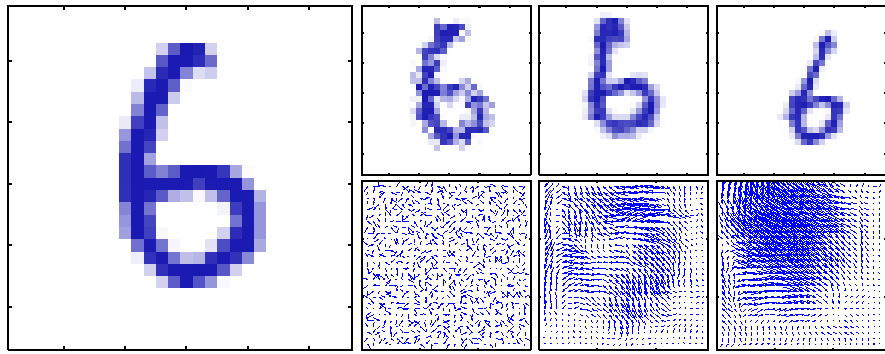
\includegraphics[width=0.65\linewidth]{./figures/Figure5_14.pdf}
        \caption{\scriptsize Synthetic warps of a digit generated by sampling random displacement fields (from \cite{bishop2006pattern}).}
    \end{figure}
\end{frame}

\begin{frame}{Not all data augmentation works}
    The effectiveness of data synthesis depends on the application.	%\pause
    \begin{itemize}
        \item In density estimation, generating new samples requires an already accurate model of the data distribution. %\pause
        \item For visual recognition tasks, data augmentation is effective because many image variations can be simulated.	%\pause
        \begin{itemize}
            \item Translating training images by a few pixels often improves generalization.	%\pause
            \item Other common transformations include rotation and scaling.	%\pause
            \item Care must be taken to avoid transformations that alter the true class.
        \end{itemize}
    \end{itemize}
\end{frame}

\begin{frame}{Injecting noise}
\begin{itemize}
    \item In many classification and regression tasks, the model should perform well even with small random noise in the input.  
    \item Neural networks are often sensitive to noise unless trained to handle it.  
    \item A simple way to improve robustness is to train with noise-injected inputs.  
\end{itemize}
\end{frame}

    \begin{frame}{Conclusion}
      \begin{itemize}
        \item Preprocessing followed by forward passes, backward passes, and testing from the classic training pipeline.
        \item Using the pipeline, artificial neural networks enable computers to make sense of images.
        \item The optimization result depends on the initialization.
        \item The initialization depends on the seed of the pseudorandom number generator.
        \item \textit{Seed-values must be recorded}, to allow reproduction.
        \item Share the results of multiple re-initialized runs, if possible.
				\item For visual recognition problems, data augmentation often improves performance of the models.
      \end{itemize}
    \end{frame}

    \begin{frame}[allowframebreaks]{Literature}
      \printbibliography
    \end{frame}
%
    %\section{Network coding}
    %\begin{frame}[fragile]{Networks in Flax}
      %Code examples for added implementation fun!! A minimal net:
      %\begin{python}
      %import jax.numpy as jnp
      %from flax import linen as nn
%
      %class Net(nn.Module):
      %@nn.compact
      %def __call__(self, x):
          %x = jnp.reshape(x,
              %[x.shape[0], -1])
          %x = nn.Dense(10)(x)
          %x = nn.sigmoid(x)
          %return x
      %\end{python}
      %Add more layers in our own experiments!!
    %\end{frame}
%
    %\begin{frame}[fragile]{Network initialization}
      %Initialization requires a key for the pseudorandom number generator.
      %\begin{python}
      %key = jax.random.PRNGKey(key)
      %net = Net()
      %variables = net.init(
          %key, jnp.ones([batch_size]
          %+ list(img_data_train.shape[1:])
          %+ [1])
      %)
      %\end{python} 
    %\end{frame}
%
    %\begin{frame}[fragile]{A forward pass}
      %A forward pass through the net requires the weights and an input array.
      %\begin{python}
      %output = net.apply(
        %variables,
        %jnp.expand_dims(img_batch, -1)
      %)
      %\end{python}
    %\end{frame}
%
    %\begin{frame}[fragile]{Gradient steps on weight trees} 
      %\begin{python}
      %weights = jax.tree_util.tree_map(
          %update_fun,
          %weights, grads
      %)
      %\end{python} 
      %It's useful to use a lambda function here.
      %The function should have two arguments \texttt{weights} and \texttt{grads} and return
      %\texttt{weights} - \texttt{learning\_rate * grads}. \\
      %More information on lambda functions: \\
      %\url{https://docs.python.org/3/tutorial/controlflow.html#lambda-expressions} . \\
      %More information on the tree maps: \\
      %\url{https://jax.readthedocs.io/en/latest/_autosummary/jax.tree_util.tree_map.html}
    %\end{frame}

\end{document}
